
\documentclass[aspectratio=169]{beamer}
\setbeamertemplate{navigation symbols}{}

\usepackage{subfigure,epsfig,amsfonts}
\usepackage{beamerthemeshadow}
\usepackage{amsmath}
\usepackage{bm}
\usepackage{siunitx}


\setbeamertemplate{footline}{}
\setbeamertemplate{navigation symbols}{}
\setbeamertemplate{headline}
{%
  \leavevmode%
  \begin{beamercolorbox}[wd=.5\paperwidth,ht=2.5ex,dp=1.125ex]{section in head/foot}%
    \hbox to .5\paperwidth{\hfil\insertsectionhead\hfil}
  \end{beamercolorbox}%
  \begin{beamercolorbox}[wd=.5\paperwidth,ht=2.5ex,dp=1.125ex]{subsection in head/foot}%
    \hbox to .5\paperwidth{\hfil\insertsubsectionhead\hfil}
  \end{beamercolorbox}%
}

\begin{document}
\title{Statistical inference and memory in recurrent networks of spiking neurons}  
\author{Clayton Seitz}
\date{\today} 

\maketitle


\begin{frame}{Outline}
\tableofcontents
\end{frame}

\section{A short note on deep learning}

\begin{frame}{A brief survey of deep learning architectures}

\begin{itemize}
\item Perceptrons e.g. MLPs for classification of vectorized data
\item Convolutional neural networks (CNNs) for image classification, segmentation
\item Recurrent neural networks (RNNs) for temporal data
\item Generative adversarial networks (GANs) and autoencoders e.g. VAEs for generative modeling
\item ...
\end{itemize}

\vfill
{\color{red} which are all trained offline on known samples from some (perhaps very complicated) population distribution}

\end{frame}

\begin{frame}{Review of Bayesian inference}

Recall Bayes theorem from fundamental probability theory

\begin{equation*}
P(A|B) = \frac{P(B|A)P(A)}{P(B)} = \frac{P(B|A)P(A)}{\int P(B|A)P(A)dA}
\end{equation*}
\vfill

$P(A|B)$ is called the posterior, $P(B|A)$ the likelihood, $P(A)$ the prior, and $P(B)$ the evidence
\vfill

\begin{equation*}
P(B) = \int P(B|A)P(A)dA
\end{equation*}

Calculating this integral is often intractable. Monte-Carlo Markov Chain (MCMC) methods and variational inference offer solutions

\end{frame}

\section{Deep generative models}
\begin{frame}{Deep generative models: variational autoencoders (VAEs)}

\begin{figure}
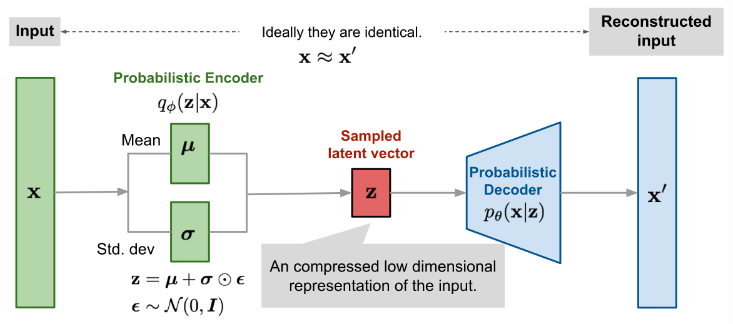
\includegraphics[width=135mm]{vae-diagram}
\end{figure}

The VAE \emph{approximates} the true posterior $P(Z|X)$ with a neural network

\end{frame}

\begin{frame}{Deep generative models: variational autoencoders (VAE)}

When training a VAE we're concerned with the following problem:

$$\min_{\phi} \,\ \mathbb E_{x \sim Pop, z \sim P_\phi(z|x)} \left[ \ln \frac{P_\phi(z|x)}{P(z)} - \ln P_\phi(x|z) \right] \,.$$

We can model $P_\phi(z|x)$ with an encoder and $P_\phi(x|z)$ with a decoder as follows:
$$P_\phi(z|x) = \mathcal N \left(\mu_{\phi,z}(x), \Sigma_{\phi,z}(x) \right)$$
$$P_\phi(x|z) = \mathcal N \left( \mu_{\phi,x}(z), \sigma^2 I \right) \,,$$
where $\mu_{\phi,z}, \Sigma_{\phi,z}, \mu_{\phi,x}$ are neural networks, and $\Sigma_{\phi,z}(x)$ is diagonal.
\vfill
Let $P(z)$ (the prior over $z$) to be $\mathcal N(0, I)$.


\end{frame}

\begin{frame}{Using Monte-Carlo Markov Chain (MCMC) to sample the posterior}

Monte Carlo methods estimate distributions by repeated sampling

\vfill
If calculating $P(B)$ is intractable and we require samples from the posterior $P(A|B )$ we can use MCMC
\vfill
A prominent hypothesis in neuroscience is that neurons use 

\end{frame}

\begin{frame}{SNNs can run on emerging dedicated hardware}

\begin{itemize}
\item The entire brain is estimated consume 10W of power
\item Spiking networks (SNNs) perform computations in memory giving low-latency
\item SNNs can in principle self-organize without backprop (unsupervised learning)
\end{itemize}

\begin{figure}
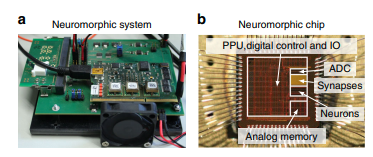
\includegraphics[width=110mm]{hardware-figure}
\end{figure}

\end{frame}

\begin{frame}{SNNs can encode information in the phase of neural responses}
Thus a coding of analog variables by firing rates seems quite dubious in the context of fast cortical computations 

\end{frame}

\section{Biologically inspired neural networks}
\begin{frame}{The third generation of neural networks: spiking nets}

\begin{columns}
\column{0.5\linewidth}
\begin{figure}
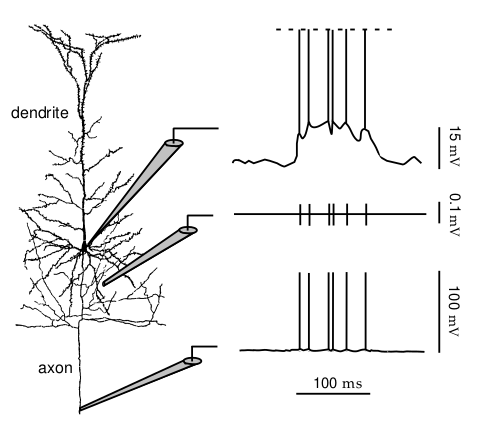
\includegraphics[height=55mm, width=75mm]{figure-18}
\end{figure}
\column{0.5\linewidth}
\begin{itemize}
\item $\sim$ 16 billion neurons in cortex
\item A neuron receives on the order of $10^{3}$ to $10^{4}$ synaptic inputs
\item Neurons communicate via action potentials in an all-or-nothing fashion
\end{itemize}

\end{columns} 

\end{frame}

\begin{frame}{The third generation of neural networks: spiking nets}

\begin{itemize}
\item Post-synaptic potentials (PSPs) allow pre-synaptic action potentials to change post-synaptic membrane potential
\item PSPs can be positive or negative (excitatory or inhibitory)
\end{itemize}


\end{frame}

\begin{frame}{Integrate and fire (IF) neuron models}

\begin{figure}
\centering
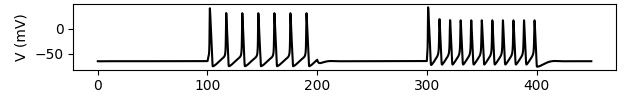
\includegraphics[width=140mm]{figure-19-1}
\end{figure}

\begin{figure}
\centering
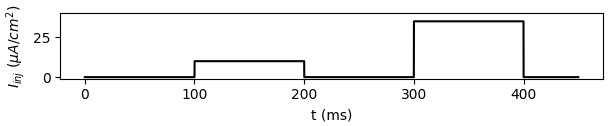
\includegraphics[width=140mm]{figure-19-2}
\end{figure}

\begin{equation*}
\tau\dot{V}(t) = g_{\ell}(E - V) + g_{\ell}\cdot \psi(V) + I(t)
\end{equation*}


\end{frame}

\begin{frame}{Monte-Carlo simulation of uncoupled IF neurons}

When $\psi(V) = g_{\ell}\Delta_{T}\exp\left(\frac{V-V_{L}}{\Delta_{T}}\right)$ we have the exponential integrate and fire model

\begin{figure}
\centering
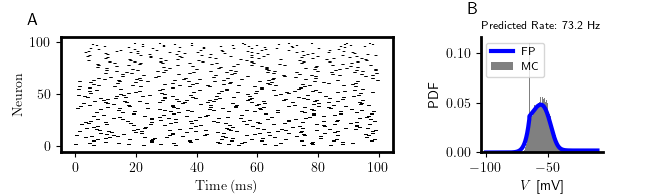
\includegraphics[width=140mm]{figure-3-1}
\end{figure}

Langevin equations have a corresponding Fokker-Planck equation 

\begin{equation*}
\frac{\partial P}{\partial t} = \frac{\sigma^{2}}{\tau}\frac{\partial^{2}P}{\partial V^{2}} + \frac{\partial}{\partial V}\left(\frac{V-E+\psi}{\tau}P\right)
\end{equation*}

\end{frame}


\begin{frame}{Synaptic coupling can induce correlations in spiking activity}

For special synaptic connectivity regimes dynamical variables can remain uncorrelated between neurons

\begin{figure}
\centering
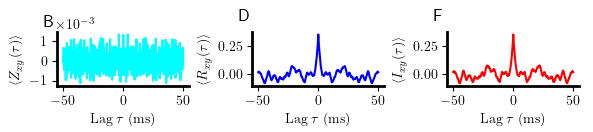
\includegraphics[width=140mm]{figure-12-1}
\end{figure}

Uncorrelated neural activity captures irregular spiking seen \emph{in-vivo}

\end{frame}

\section{Synaptic connectivity as an internal model}
\begin{frame}{Predicting neuron correlations}
The linear response of $r(t)$ allows us to also estimate the matrix of cross-correlations $C_{kj}(\tau)$
from the synaptic connectivity $\mathcal{C}$
\begin{figure}
\centering
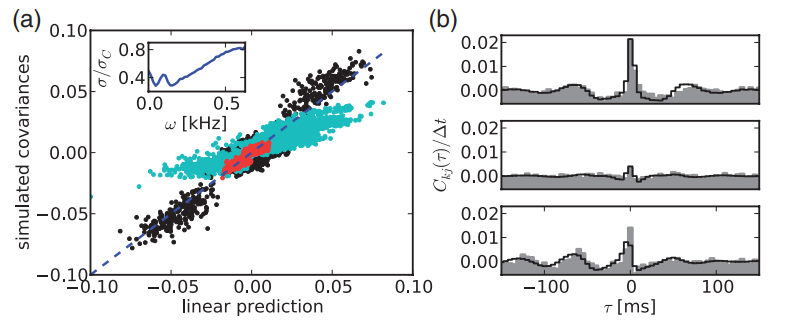
\includegraphics[width=110mm]{figure-20}
\end{figure}

This has important implications for brain-inspired machine learning

\end{frame}


\end{document}